\documentclass{./civarticle}
\usepackage{graphicx} % Required for inserting images

\title{Эссе по теме "Блоковые шифры"}
\author{Костиков Егор Вячеславович}
\date{Январь 2024}

\begin{document}

\maketitle

\section{Введение}

В данной работе приводится описание основных блоковых шифров: описываются шифры DES, 3DES, AES, ГОСТ 34.12-2018 Магма, ГОСТ 34.12-2018 Кузнечик, IDEA, IDEA NXT и RC6. Также приводится более подробное описание и анализ шифра AES.

\section{Термины и определения}

Симметричная криптосистема (симметричные шифр) --- способ шифрования, в котором для шифрования и расшифрования применяется один и тот же криптографический ключ.

Потоковый шифр ---  симметричный шифр, оперирующий (шифрующий) группами бит фиксированной длины --- блоками.

Регистр сдвига с линейной обратной связью --- сдвиговый регистр битовых слов, у которого значение входного бита однозначно задается некоторой функцией, исходя из значений остальных битов регистра до сдвига.

S-блок ---  функция в коде программы или аппаратная система, принимающая на входе n бит, преобразующая их по определённому алгоритму и возвращающая на выходе m бит.

Далее в работе используются следующие обозначения:
\begin{itemize}
    \item $X <<< n$ --- сдвиг содержимого $X$ на $n$ бит влево;
    \item $X >>> n$ --- сдвиг содержимого $X$ на $n$ бит вправо;
    \item $x \mathbin\Vert y$ --- конкатенация строк $x$ и $y$;
    \item $=$, $\leftarrow$ --- операторы присваивания;
    \item $x \oplus y$ --- побитовое сложение $x$ и $y$;
    \item $x \boxplus y$ --- сложение $x$ и $y$ по модулю $2^{32}$ (для шифра IDEA --- по модулю $2^{16}$);
    \item $\odot$ --- операция умножения по модулю $2^{16} + 1$, вместо нуля используется значение $2^{16}$.
\end{itemize}

\section{Описание основных блоковых шифров}

\subsection{Шифры DES и 3DES}

\subsubsection{Шифр DES}

Описание блокового шифра DES приводится в соответствии со спецификацией данного шифра, описанной в \cite{des}.

Размеры блока данных $T$ для шифрования и ключа $KEY$ равны и составляют по 64 бита (ключ $KEY$ состоит из непосредственно 56 ключевых битов и дополнительных восьми контрольных битов с номерами 8, 16, 24, 32, 40, 48, 54, 64, используемых для обнаружения возможных ошибок).

При шифровании выполняется следующая последовательность действий:
\begin{enumerate}
    \item Начальная перестановка бит блока $T$: вычисление значения $IP(T)$;
    \item Пусть $L_0$ и $R_0$ 32-битные блоки, на которые разбивается $IP(T)$: $IP(T) = L_0 \mathbin\Vert R_0$;
    \item $For$ $n$ $=$ $1$ $to$ $16$ $do$ \{ 

    \hspace{0.5cm} $K_n = KS(n, KEY)$;
    
    \hspace{0.5cm} $L_n = R_{n-1}$;

    \hspace{0.5cm} $R_n = L_{n-1} \oplus f(R_{n-1}, K_n)$;
    
\}
    \item Зашифрованный блок $CT$ определяется путем применения перестановки $IP^{-1}$: $CT = IP^{-1}(R_{16} \mathbin\Vert L_{16})$.
\end{enumerate}

При расшифровании выполняется следующая последовательность действий:

\begin{enumerate}
    \item Начальная перестановка бит блока $CT$: вычисление значения $IP(CT)$;
    \item Пусть $R_{16}$ и $L_{16}$ 32-битные блоки, на которые разбивается $IP(CT)$: $IP(CT) = R_{16} \mathbin\Vert L_{16}$;
    \item $For$ $n$ $=$ $16$ $downto$ $1$ $do$ \{ 

    \hspace{0.5cm} $K_n = KS(n, KEY)$;
    
    \hspace{0.5cm} $R_{n-1} = L_{n}$;

    \hspace{0.5cm} $L_{n-1} = R_{n} \oplus f(L_{n}, K_n)$;
    
\}

    \item Расшифрованный блок $T$ определяется путем применения перестановки $IP^{-1}$: $T = IP^{-1}(L_{0} \mathbin\Vert R_{0})$.

\end{enumerate}

Описание компонентов шифра:
\begin{itemize}
    \item Начальная перестановка $IP$ (Initial Permutation) битов исходного блока $T$ задается следующей таблицей:

\begin{longtable}{|p{0.5cm}|p{0.5cm}|p{0.5cm}|p{0.5cm}|p{0.5cm}|p{0.5cm}|p{0.5cm}|p{0.5cm}|}
\hline
58 & 50 & 42 & 34 & 26 & 18 & 10 & 2 \\
\hline
60 & 52 & 44 & 36 & 28 & 20 & 12 & 4 \\
\hline
62 & 54 & 46 & 38 & 30 & 22 & 14 & 6 \\
\hline
64 & 56 & 48 & 40 & 32 & 24 & 16 & 8 \\
\hline
57 & 49 & 41 & 33 & 25 & 17 & 9 & 1 \\
\hline
59 & 51 & 43 & 35 & 27 & 19 & 11 & 3 \\
\hline
61 & 53 & 45 & 37 & 29 & 21 & 13 & 5 \\
\hline
63 & 55 & 47 & 39 & 31 & 23 & 15 & 7 \\
\hline
\caption{Таблица перестановки IP}
\end{longtable}

В результате применения данной перестановки первыми тремя битами 64-битного блока $IP(T)$ будут являться биты $T$ с номерами 58, 50 и 42, а тремя последними --- биты $T$ с номерами 23, 15 и 7.

\item Функция $KS$ принимает два параметра --- номер $1 \leq n \leq 16$ и 64-битный ключ $KEY$ --- и возвращает 48-битный блок $K_n$.

\begin{enumerate}
    \item Выбор 28-битных блоков $C_0$ и $D_0$, составленных из битов ключа $KEY$ с использованием таблицы $PC$-1, имеющей следующий вид:

    \begin{longtable}{|p{0.5cm}|p{0.5cm}|p{0.5cm}|p{0.5cm}|p{0.5cm}|p{0.5cm}|p{0.5cm}|}
\hline
57 & 49 & 41 & 33 & 25 & 17 & 9 \\
\hline
1 & 58 & 50 & 42 & 34 & 26 & 18 \\
\hline
10 & 2 & 59 & 51 & 43 & 35 & 27 \\
\hline
19 & 11 & 3 & 60 & 52 & 44 & 36 \\
\hline
63 & 55 & 47 & 39 & 31 & 23 & 15 \\
\hline
7 & 62 & 54 & 46 & 38 & 30 & 22 \\
\hline
14 & 6 & 61 & 53 & 45 & 37 & 29 \\
\hline
21 & 13 & 5 & 28 & 20 & 12 & 4 \\
\hline
\caption{Таблица $PC$-1}
\end{longtable}

Первые четыре строки определяют содержимое блока $C_0$: первыми тремя битами $C_0$ являются 57, 49 и 41 биты ключа $KEY$, а тремя последними --- 52, 44 и 36. Последние четыре строки определяют содержмое блока $D_0$: первыми тремя битами $D_0$ являются 63, 55 и 47 биты ключа $KEY$, а тремя последними --- 20, 12 и 4. 

\item Посредством левых циклических сдвигов содержимого $C_{i-1}$ и $D_{i-1}$ происходит получение значений $C_i$ и $D_i$ соответственно, где $1 \leq i \leq n \leq 16$. Количество сдвигов варьируется от одного до двух и определяется исходя из номера текущей итерации: 

\begin{longtable}{|p{1cm}|p{0.5cm}|p{0.5cm}|p{0.5cm}|p{0.5cm}|p{0.5cm}|p{0.5cm}|p{0.5cm}|p{0.5cm}|p{0.5cm}|p{0.5cm}|p{0.5cm}|p{0.5cm}|p{0.5cm}|p{0.5cm}|p{0.5cm}|p{0.5cm}|}
\hline
Номер итерации & 1 & 2 & 3 & 4 & 5 & 6 & 7 & 8 & 9 & 10 & 11 & 12 & 13 & 14 & 15 & 16 \\
\hline
Число сдвигов & 1 & 1 & 2 & 2 & 2 & 2 & 2 & 2 & 1 & 2 & 2 & 2 & 2 & 2 & 2 & 1 \\
\hline
\caption{Таблица определения количества сдвигов}
\end{longtable}

\item После этого из битов содержимого $C_n \mathbin\Vert D_n$ происходит выбор 48 битов, составляющих блок $K_n$. Выбор происходит на основе таблицы $PC$-2:

\begin{longtable}{|p{0.5cm}|p{0.5cm}|p{0.5cm}|p{0.5cm}|p{0.5cm}|p{0.5cm}|}
\hline
14 & 17 & 11 & 24 & 1 & 5 \\
\hline
3 & 28 & 15 & 6 & 21 & 10 \\
\hline
23 & 19 & 12 & 4 & 26 & 8 \\
\hline
16 & 7 & 27 & 20 & 13 & 2 \\
\hline
41 & 52 & 31 & 37 & 47 & 55 \\
\hline
30 & 40 & 51 & 45 & 33 & 48 \\
\hline
44 & 49 & 39 & 56 & 34 & 53 \\
\hline
46 & 42 & 50 & 36 & 29 & 32 \\
\hline
\caption{Таблица $PC$-2}
\end{longtable}

Согласно данной таблице, первыми тремя битами $K_n$ являются 14, 17 и 11 биты $C_n \mathbin\Vert D_n$, а тремя последними --- 36, 29 и 32 биты $C_n \mathbin D_n$.


\end{enumerate}

\item Функция $f$ принимает два параметра --- 32-битный блок $R_{n-1}$ и 48-битный блок $K_n$ --- и возвращает 32-битный блок $R_n$. Функция выполняется следующим образом: 

\begin{enumerate}
    \item Параметр $R_{n-1}$ подается на вход функции $E$, которая переводит 32-битный блок в 48-битный блок $E(R_{n-1})$ посредством дублирования некоторых битов входного блока. Функция $E$ определяется следующей таблицей:

    \begin{longtable}{|p{0.5cm}|p{0.5cm}|p{0.5cm}|p{0.5cm}|p{0.5cm}|p{0.5cm}|}
\hline
32 & 1 & 2 & 3 & 4 & 5 \\
\hline
4 & 5 & 6 & 7 & 8 & 9 \\
\hline
8 & 9 & 10 & 11 & 12 & 13 \\
\hline
12 & 13 & 14 & 15 & 16 & 17 \\
\hline
16 & 17 & 18 & 19 & 20 & 21 \\
\hline
20 & 21 & 22 & 23 & 24 & 25 \\
\hline
24 & 25 & 26 & 27 & 28 & 29 \\
\hline
28 & 29 & 30 & 31 & 32 & 1 \\
\hline
\caption{Таблица расширения функции $E$}
\end{longtable}

Согласно данной таблице, первыми тремя битами $E(R_{n-1})$ являются 32, 1 и 2 биты блока $R_{n-1}$, а последние три бита $E(R_{n-1})$ --- биты 31, 32 и 1 блока $R_{n-1}$. При этом в результирующем блоке дублируются биты 1, 4, 5, 8, 9, 12, 13, 16, 17, 20, 21, 24, 25, 28, 29, 32 блока $R_{n-1}$.

\item Значение $E(R_{n-1})$ складывается со вторым параметров функции $f$: $E(R_{n_1}) \oplus K_n$ = $B_1 \mathbin\Vert ... \mathbin\Vert B_8$, где $B_1$, ..., $B_8$ --- 6-битные блоки.

\item Восемь 6-битных блоков $B_1$, ... $B_8$ преобразуются в восемь 4-битных блоков $S_1(B_1)$, ..., $S_8(B_8)$ с использованием таблиц $S_1, ..., S_8$. Преобразование блока $B_r$ посредством таблицы $S_r$ осуществляется по следующему правилу: 
\begin{enumerate}
    \item старший и младший биты $B_r$ образуют двоичную запись числа $0 \leq i \leq 3$;
    \item оставшиеся биты $B_r$ образуют двоичную запись числа $0 \leq j \leq 15$;
    \item выбирается число $0 \leq S \leq 15$, стоящее на пересечении $i$-ой строки и $j$-го столбца таблицы $S_r$(нумерация строк и столбцов начинается с нуля); результатом $S_r(B_r)$ является двоичная запись числа $S$.
\end{enumerate}

Таблицы $S_1, ..., S_8$ имеют следующий вид:

\begin{longtable}{|p{0.5cm}|p{0.5cm}|p{0.5cm}|p{0.5cm}|p{0.5cm}|p{0.5cm}|p{0.5cm}|p{0.5cm}|p{0.5cm}|p{0.5cm}|p{0.5cm}|p{0.5cm}|p{0.5cm}|p{0.5cm}|p{0.5cm}|p{0.5cm}|}
\hline
14 & 4 & 13 & 1 & 2 & 15 & 11 & 8 & 3 & 10 & 6 & 12 & 5 & 9 & 0 & 7 \\
\hline
0 & 15 & 7 & 4 & 14 & 2 & 13 & 1 & 10 & 6 & 12 & 11 & 9 & 5 & 3 & 8 \\
\hline
4 & 1 & 14 & 8 & 13 & 6 & 2 & 11 & 15 & 12 & 9 & 7 & 3 & 10 & 5 & 0 \\
\hline
15 & 12 & 8 & 2 & 4 & 9 & 1 & 7 & 5 & 11 & 3 & 14 & 10 & 0 & 6 & 13 \\
\hline
\caption{Таблица $S_1$}
\end{longtable}

\begin{longtable}{|p{0.5cm}|p{0.5cm}|p{0.5cm}|p{0.5cm}|p{0.5cm}|p{0.5cm}|p{0.5cm}|p{0.5cm}|p{0.5cm}|p{0.5cm}|p{0.5cm}|p{0.5cm}|p{0.5cm}|p{0.5cm}|p{0.5cm}|p{0.5cm}|}
\hline
15 & 1 & 8 & 14 & 6 & 11 & 3 & 4 & 9 & 7 & 2 & 13 & 12 & 0 & 5 & 10 \\
\hline
3 & 13 & 4 & 7 & 15 & 2 & 8 & 14 & 12 & 0 & 1 & 10 & 6 & 9 & 11 & 5 \\
\hline
0 & 14 & 7 & 11 & 10 & 4 & 13 & 1 & 5 & 8 & 12 & 6 & 9 & 3 & 2 & 15 \\
\hline
13 & 8 & 10 & 1 & 3 & 15 & 4 & 2 & 11 & 6 & 7 & 12 & 0 & 5 & 14 & 9 \\
\hline
\caption{Таблица $S_2$}
\end{longtable}

\begin{longtable}{|p{0.5cm}|p{0.5cm}|p{0.5cm}|p{0.5cm}|p{0.5cm}|p{0.5cm}|p{0.5cm}|p{0.5cm}|p{0.5cm}|p{0.5cm}|p{0.5cm}|p{0.5cm}|p{0.5cm}|p{0.5cm}|p{0.5cm}|p{0.5cm}|}
\hline
10 & 0 & 9 & 14 & 6 & 3 & 15 & 5 & 1 & 13 & 12 & 7 & 11 & 4 & 2 & 8 \\
\hline
13 & 7 & 0 & 9 & 3 & 4 & 6 & 10 & 2 & 8 & 5 & 14 & 12 & 11 & 15 & 1 \\
\hline
13 & 6 & 4 & 9 & 8 & 15 & 3 & 0 & 11 & 1 & 2 & 12 & 5 & 10 & 14 & 7 \\
\hline
1 & 10 & 13 & 0 & 6 & 9 & 8 & 7 & 4 & 15 & 14 & 3 & 11 & 5 & 2 & 12 \\
\hline
\caption{Таблица $S_3$}
\end{longtable}

\begin{longtable}{|p{0.5cm}|p{0.5cm}|p{0.5cm}|p{0.5cm}|p{0.5cm}|p{0.5cm}|p{0.5cm}|p{0.5cm}|p{0.5cm}|p{0.5cm}|p{0.5cm}|p{0.5cm}|p{0.5cm}|p{0.5cm}|p{0.5cm}|p{0.5cm}|}
\hline
7 & 13 & 14 & 3 & 0 & 6 & 9 & 10 & 1 & 2 & 8 & 5 & 11 & 12 & 4 & 15 \\
\hline
13 & 8 & 11 & 5 & 6 & 15 & 0 & 3 & 4 & 7 & 2 & 12 & 1 & 10 & 14 & 9 \\
\hline
10 & 6 & 9 & 0 & 12 & 11 & 7 & 13 & 15 & 1 & 3 & 14 & 5 & 2 & 8 & 4 \\
\hline
3 & 15 & 0 & 6 & 10 & 1 & 13 & 8 & 9 & 4 & 5 & 11 & 12 & 7 & 2 & 14 \\
\hline
\caption{Таблица $S_4$}
\end{longtable}

\begin{longtable}{|p{0.5cm}|p{0.5cm}|p{0.5cm}|p{0.5cm}|p{0.5cm}|p{0.5cm}|p{0.5cm}|p{0.5cm}|p{0.5cm}|p{0.5cm}|p{0.5cm}|p{0.5cm}|p{0.5cm}|p{0.5cm}|p{0.5cm}|p{0.5cm}|}
\hline
2 & 12 & 4 & 1 & 7 & 10 & 11 & 6 & 8 & 5 & 3 & 15 & 13 & 0 & 14 & 9 \\
\hline
14 & 11 & 2 & 12 & 4 & 7 & 13 & 1 & 5 & 0 & 15 & 10 & 3 & 9 & 8 & 6 \\
\hline
4 & 2 & 1 & 11 & 10 & 13 & 7 & 8 & 15 & 9 & 12 & 5 & 6 & 3 & 0 & 14 \\
\hline
11 & 8 & 12 & 7 & 1 & 14 & 2 & 13 & 6 & 15 & 0 & 9 & 10 & 4 & 5 & 3 \\
\hline
\caption{Таблица $S_5$}
\end{longtable}

\begin{longtable}{|p{0.5cm}|p{0.5cm}|p{0.5cm}|p{0.5cm}|p{0.5cm}|p{0.5cm}|p{0.5cm}|p{0.5cm}|p{0.5cm}|p{0.5cm}|p{0.5cm}|p{0.5cm}|p{0.5cm}|p{0.5cm}|p{0.5cm}|p{0.5cm}|}
\hline
12 & 1 & 10 & 15 & 9 & 2 & 6 & 8 & 0 & 13 & 3 & 4 & 14 & 7 & 5 & 11 \\
\hline
10 & 15 & 4 & 2 & 7 & 12 & 9 & 5 & 6 & 1 & 13 & 14 & 0 & 11 & 3 & 8 \\
\hline
9 & 14 & 15 & 5 & 2 & 8 & 12 & 3 & 7 & 0 & 4 & 10 & 1 & 13 & 11 & 6 \\
\hline
4 & 3 & 2 & 12 & 9 & 5 & 15 & 10 & 11 & 14 & 1 & 7 & 6 & 0 & 8 & 13 \\
\hline
\caption{Таблица $S_6$}
\end{longtable}

\begin{longtable}{|p{0.5cm}|p{0.5cm}|p{0.5cm}|p{0.5cm}|p{0.5cm}|p{0.5cm}|p{0.5cm}|p{0.5cm}|p{0.5cm}|p{0.5cm}|p{0.5cm}|p{0.5cm}|p{0.5cm}|p{0.5cm}|p{0.5cm}|p{0.5cm}|}
\hline
4 & 11 & 2 & 14 & 15 & 0 & 8 & 13 & 3 & 12 & 9 & 7 & 5 & 10 & 6 & 1 \\
\hline
13 & 0 & 11 & 7 & 4 & 9 & 1 & 10 & 14 & 3 & 5 & 12 & 2 & 15 & 8 & 6 \\
\hline
1 & 4 & 11 & 13 & 12 & 3 & 7 & 14 & 10 & 15 & 6 & 8 & 0 & 5 & 9 & 2 \\
\hline
6 & 11 & 13 & 8 & 1 & 4 & 10 & 7 & 9 & 5 & 0 & 15 & 14 & 2 & 3 & 12 \\
\hline
\caption{Таблица $S_7$}
\end{longtable}

\begin{longtable}{|p{0.5cm}|p{0.5cm}|p{0.5cm}|p{0.5cm}|p{0.5cm}|p{0.5cm}|p{0.5cm}|p{0.5cm}|p{0.5cm}|p{0.5cm}|p{0.5cm}|p{0.5cm}|p{0.5cm}|p{0.5cm}|p{0.5cm}|p{0.5cm}|}
\hline
13 & 2 & 8 & 4 & 6 & 15 & 11 & 1 & 10 & 9 & 3 & 14 & 5 & 0 & 12 & 7 \\
\hline
1 & 15 & 13 & 8 & 10 & 3 & 7 & 4 & 12 & 5 & 6 & 11 & 0 & 14 & 9 & 2 \\
\hline
7 & 11 & 4 & 1 & 9 & 12 & 14 & 2 & 0 & 6 & 10 & 13 & 15 & 3 & 5 & 8 \\
\hline
2 & 1 & 14 & 7 & 4 & 10 & 8 & 13 & 15 & 12 & 9 & 0 & 3 & 5 & 6 & 11 \\
\hline
\caption{Таблица $S_8$}
\end{longtable}

\item Производится еще одна перестановка с помощью функции $P$, принимающей на вход 32-битный блок $S_1(B_1) \mathbin\Vert ... \mathbin\Vert S_8(B_8)$, которая задается следующей таблицей:

\begin{longtable}{|p{0.5cm}|p{0.5cm}|p{0.5cm}|p{0.5cm}|}
\hline
16 & 7 & 20 & 21 \\
\hline
29 & 12 & 28 & 17 \\
\hline
1 & 15 & 23 & 26 \\
\hline
5 & 18 & 31 & 10 \\
\hline
2 & 8 & 24 & 14 \\
\hline
32 & 27 & 3 & 9 \\
\hline
19 & 13 & 30 & 6 \\
\hline
22 & 11 & 4 & 25 \\
\hline
\caption{Таблица перестановки $P$}
\end{longtable}

Согласно данной таблице, первыми тремя битами $P(S_1(B_1) \mathbin\Vert ... \mathbin\Vert S_8(B_8))$ являются 16, 7 и 20 биты слова $S_1(B_1) \mathbin\Vert ... \mathbin\Vert S_8(B_8)$, а тремя последними --- 11, 4 и 25 биты слова $S_1(B_1) \mathbin\Vert ... \mathbin\Vert S_8(B_8)$.

\item Функцией $f(R_{n-1}, K_n)$ возвращается значение $P(S_1(B_1) \mathbin\Vert ... \mathbin\Vert S_8(B_8))$.
    
\end{enumerate}


\item Обратная перестановка $IP^{-1}$ битов блока $T$ задается следующей таблицей:

\begin{longtable}{|p{0.5cm}|p{0.5cm}|p{0.5cm}|p{0.5cm}|p{0.5cm}|p{0.5cm}|p{0.5cm}|p{0.5cm}|}
\hline
40 & 8 & 48 & 16 & 56 & 24 & 64 & 32 \\
\hline
39 & 7 & 47 & 15 & 55 & 23 & 63 & 31 \\
\hline
38 & 6 & 46 & 14 & 54 & 22 & 62 & 30 \\
\hline
37 & 5 & 45 & 13 & 53 & 21 & 61 & 29 \\
\hline
36 & 4 & 44 & 12 & 52 & 20 & 60 & 28 \\
\hline
35 & 3 & 43 & 11 & 51 & 19 & 59 & 27 \\
\hline
34 & 2 & 42 & 10 & 50 & 18 & 58 & 26 \\
\hline
33 & 1 & 41 & 9 & 49 & 17 & 57 & 25 \\
\hline
\caption{Таблица перестановки $IP^{-1}$}
\end{longtable}

В результате применения данной перестановки первыми тремя битами 64-битного блока $IP^{-1}(T)$ будут являться биты $T$ с номерами 40, 8 и 48, а тремя последними --- биты $T$ с номерами 17, 57 и 25.

\end{itemize}



\subsubsection{Шифр 3DES}

Описание блокового шифра 3DES приводится в соответствии со спецификацией данного шифра, описанной в \cite{3des}.

Шифр 3DES (Triple DES, Triple Data Encryption Algorithm) основан на использовании шифра DES: для шифрования к каждому блоку данных трижды применяется алгоритм шифрования DES.

Обозначим через $E_K(I)$ результат шифрования 64-битного блока $I$ с помощью алгоритма шифрования DES с использованием ключа $K$, а через $D_K(I)$ --- результат расшифрования 64-битного блока $I$ с помощью алгоритма расшифрования DES с использованием ключа $K$. Тогда:
\begin{itemize}
    \item Шифрование 64-битного блока $I$ посредством шифра 3DES реализуется следующим образом:\\ $O = E_{K_3}(D_{K_2}(E_{K_1}(I)))$;
    \item Расшифрование 64-битного блока $O$ посредством шифра 3DES реализуется следующим образом:\\ $I = D_{K_1}(E_{K_2}(D_{K_3}(O)))$.
\end{itemize}

При этом используемые ключи могут быть выбраны одним из следующих образов:
\begin{enumerate}
    \item $K_1, K_2, K_3$ --- независимые ключи;
    \item $K_1, K_2$ --- независимые ключи, $K_3 = K_1$;
    \item $K_1 = K_2 = K_3$.
\end{enumerate}

\subsection{Шифр AES}

\subsubsection{Описание шифра}

Описание шифра приводится в соответствии с описанием, приведенным в стандарте \cite{aesdesc}.

Длина входного блока, с которым работает данный шифр, составляет 128 бит, длина ключа --- 128, 192 или 256 бит.

При шифровании 128-битного блока $T$ происходит $N_r$ итераций шифрования, где значение $N_r$ определяется в зависимости от длины используемого ключа: 128 бит --- $N_r = 10$, 192 бита --- $N_r = 12$, 256 бит --- $N_r = 14$. При этом выполняется следующая последовательность действий:
\begin{enumerate}
    \item STATE = $T$;

    \item AddRoundKey(STATE, w[0, 3]);

    \item $For$ $round$ $=$ $1$ $to$ $N_r - 1$ $do$ \{ 

    \hspace{0.5cm} SubBytes(STATE);

    \hspace{0.5cm} ShiftRows(STATE);

    \hspace{0.5cm} MixColumns(STATE);

    \hspace{0.5cm} AddRoundKey(STATE, w[$4\cdot round$, $4\cdot(round + 1) - 1$]);
    
    \}

    \item SubBytes(STATE);

    \item ShiftRows(STATE);

    \item AddRoundKey(STATE, w[$4\cdot N_r$, $4\cdot (N_r + 1) - 1$]);

    \item Зашифрованный блок $CT$ находится в состоянии STATE.
    
\end{enumerate}

В данном алгоритме через $w$ обозначен массив раундовых ключей, имеющий размер $4(N_r + 1)$ и получаемый из секретного ключа KEY.

При расшифровании 128-битного блока $CT$ происходит $N_r$ итераций расшифрования, где значение $N_r$ определяется в зависимости от длины используемого ключа: 128 бит --- $N_r = 10$, 192 бита --- $N_r = 12$, 256 бит --- $N_r = 14$. При этом выполняется следующая последовательность действий:
\begin{enumerate}
    \item STATE = $CT$;

    \item AddRoundKey(STATE, w[$4\cdot N_r$, $4\cdot (N_r + 1) - 1$]);

    \item $For$ $round$ $=$ $N_r - 1$ $downto$ $1$ $do$ \{ 

    \hspace{0.5cm} ShiftRows$^{-1}$(STATE);

    \hspace{0.5cm} SubBytes$^{-1}$(STATE);

    \hspace{0.5cm} AddRoundKey(STATE, w[$4\cdot round$, $4\cdot(round + 1) - 1$]);

    \hspace{0.5cm} MixColumns$^{-1}$(STATE);
    
    \}

    \item ShiftRows$^{-1}$(STATE);

    \item SubBytes$^{-1}$(STATE);

    \item AddRoundKey(STATE, w[0, 3]);

    \item Расшифрованный блок $T$ находится в состоянии STATE.
    
\end{enumerate}

В данном алгоритме через $w$ обозначен массив раундовых ключей, имеющий размер $4(N_r + 1)$ и получаемый из секретного ключа KEY.

Описание компонентов шифра:

Производимые операции выполняются над двумерным массивом байтов, именуемым STATE. Массив STATE состоит из 4 строк байтов, в каждой из которых содержится по 4 байта.

\begin{longtable}{|c|c|c|c|}
\hline
$S_{0, 0}$ & $S_{0, 1}$ & $S_{0, 2}$ & $S_{0, 3}$ \\
\hline
$S_{1, 0}$ & $S_{1, 1}$ & $S_{1, 2}$ & $S_{1, 3}$ \\
\hline
$S_{2, 0}$ & $S_{2, 1}$ & $S_{2, 2}$ & $S_{2, 3}$ \\
\hline
$S_{3, 0}$ & $S_{3, 1}$ & $S_{3, 2}$ & $S_{3, 3}$ \\
\hline
\caption{Массив STATE}
\end{longtable}

\begin{itemize}
    \item Функцией SubBytes реализуется преобразование содержимого ячеек состояния STATE с использованием заданного S-бокса, который представлен ниже в шестнадцатеричной записи. Содержимое выбранной ячейки представляется в шестнадцатеричной записи, первая цифра соответствует номеру строки S-бокса, вторая --- номеру столбца. Значение, находящееся на пересечении определенной строки и столбца, помещается в выбранную ячейку.

    \begin{figure}[h!]
    \center{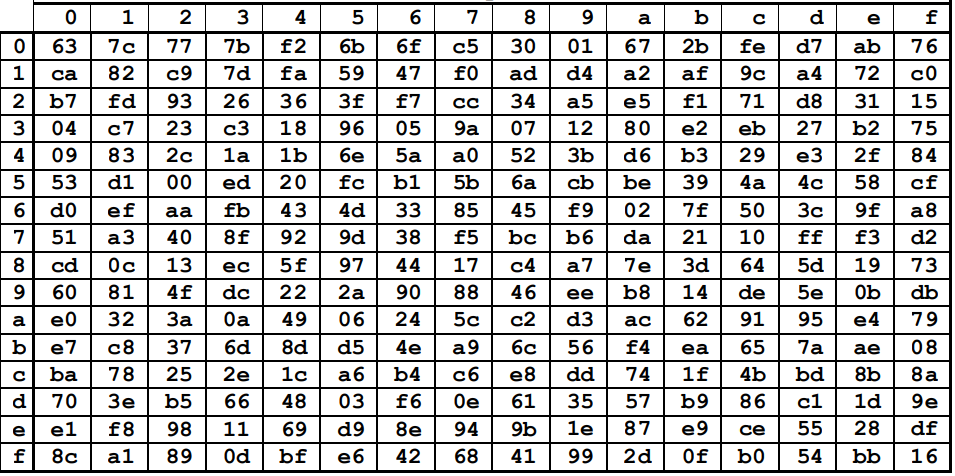
\includegraphics[width=0.5\linewidth]{sbox.png} \\ S-бокс, использующийся в функции SubBytes}
    \end{figure}

    \begin{figure}[h]
    \center{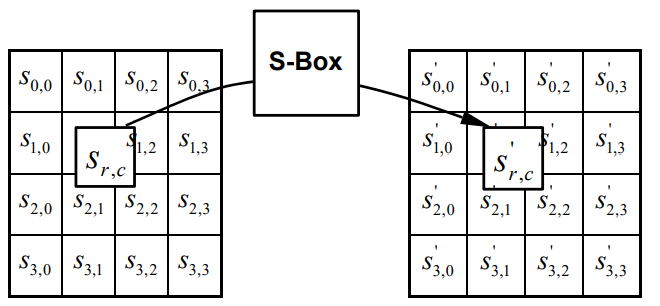
\includegraphics[width=0.5\linewidth]{subbytes.png} \\ Результат применения функции SubBytes}
    \end{figure}
    
    \item Функцией ShiftRows реализуется левый циклический сдвиг последних трех строк массива STATE: \\$S_{r,~c}~=~S_{r,~c'}$, где $c'~=~(c+r)$ mod 4, $1 \leq r \leq 3$, $0 \leq c \leq 3$. Таким образом, строка с номером 0 не сдвигается, строка с номером 1 сдвигается влево на одну позицию, строка с номером 2 сдвигается влево на две позиции, а последняя строка --- на три позиции.

    \begin{figure}[h!]
    \center{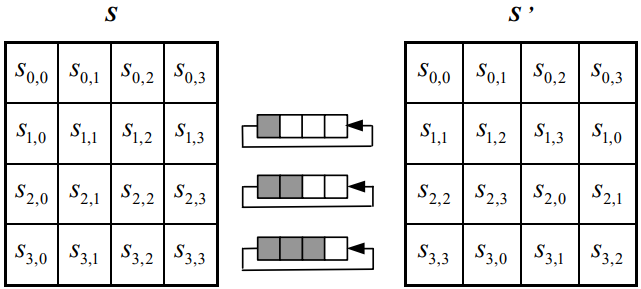
\includegraphics[width=0.5\linewidth]{shiftrows.png} \\ Результат применения функции ShiftRows}
    \end{figure}
    
    
    \item Функцией MixColumns реализуется преобразование столбцов массива STATE:

    \begin{enumerate}
        \item $s_{0, c}' = 2s_{0, c} \oplus 3s_{1, c} \oplus s_{2, c} \oplus s_{3, c}$;
        \item $s_{1, c}' = s_{0, c} \oplus 2s_{1, c} \oplus 3s_{2, c} \oplus s_{3, c}$;
        \item $s_{2, c}' = s_{0, c} \oplus s_{1, c} \oplus 2s_{2, c} \oplus 3s_{3, c}$;
        \item $s_{3, c}' = 3s_{0, c} \oplus s_{1, c} \oplus s_{2, c} \oplus 2s_{3, c}$;
    \end{enumerate}


    \begin{figure}[h!]
    \center{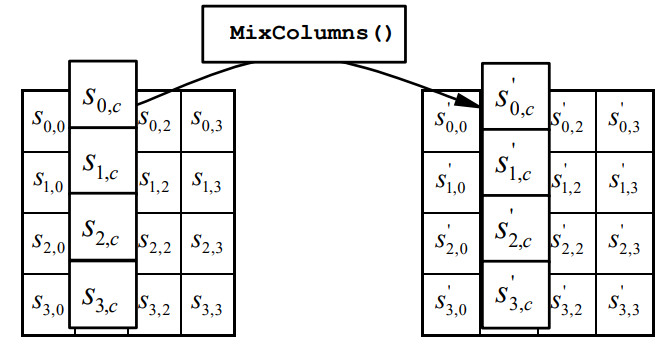
\includegraphics[width=0.5\linewidth]{mixcolumns.png} \\ Результат применения функции MixColumns}
    \end{figure}
    
    \item Функцией AddRoundKey реализуется побитовое сложение каждого байта состояния с раундовым ключом, размер которого совпадает с размером состояния STATE.

    \item Функции SubBytes, ShiftRows и MixColumns осуществляют обратимые преобразования и имеют обратные преобразования SubBytes$^{-1}$, ShiftRows$^{-1}$ и MixColumns$^{-1}$: SubBytes$^{-1}$(SubBytes(STATE)) = STATE, ShiftRows$^{-1}$(ShiftRows(STATE)) = STATE и MixColumns$^{-1}$(MixColumns(STATE)) = STATE.
\end{itemize}

\subsubsection{Анализ шифра}

В работе \cite{aes7} описывается возможность временной атаки на шифр AES, позволяющий полностью восстановить секретный ключ. Данная атака использует данные о времени выполнения каждой операции шифрования. Атака основана на том факте, что на первом раунде шифрования после применения функции AddRoundKey получаемые байты STATE $\oplus$ RoundKey используются в качестве индексов в S-блоке и могут вляить на время шифрования. Пример атаки: сбор времени, затраченного на шифрование различных входных данных $T$; суммирование времени выполнения шифра для каждого возможного значения определенного байта входного текста $T[i]$; определение значения $T[i]$, при котором суммарное время работы шифра максимально. После этого с использованием дополнительного компьютера и с тем же программным обеспечением шифра AES проивзодится перебор ключей и подбор такого секретного ключа $K$, что время работы шифра максимально при определенном значении $K[i] \oplus T[i] = M$. Затем суммируя $M \oplus T[i]$ восстанавливаем байт $K[i]$ секретного ключа, по которому возможно восстановить оставшиеся байты ключа.

В статье \cite{aes0} на основе построения коллизий описываются атаки различения и атаки восстановления ключа для шифров AES. Различители строятся на основе схемы состояния STATE шифра по истечении 4 раундов шифрования, приведенной далее.

    \begin{figure}[h!]
    \center{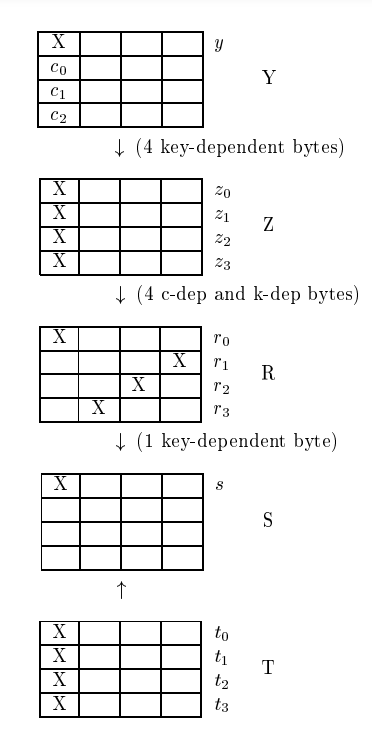
\includegraphics[width=0.4\linewidth]{image.png} \\ 4 раунда шифра}
    \end{figure}
Шифр обладает тем свойством, что если все байты перед первым раундом (Y) кроме $y$ (байт $S_{0, 0}$) фиксированы и $y$ принимается равным каждому из 256 значений, то сумма 256 результирующих значений $s$ (байт $S_{0, 0}$ после трех раундов) равна нулю. На основе данного отличительного свойства строится простейшая различительная атака, для которой необходимо $2^{32}$ открытых текстов и общей сложностью $2^{72}$.

Также предлагается четырехраундовый различитель, основанный на парадоксе дней рождения, который устроен следующим образом: выбирается набор $C$ из около $2^{16}$ триплетов $c = (c_0, c_1, c_2)$ (содержимое ячеек $S_{1, 0}, S_{2, 0}, S_{3, 0}$) и подмножество $\Lambda \subseteq \{0, ..., 255\}$, содержащее 16 возможных значений $y$.
Учитывая мощность набора $C$, с немалой вероятностью найдутся два таких различных триплета $c'$ и $c''$, что $s^{c'}[y] = s^{c''}[y]$ (через $s^{c}[y]$ обозначено значение $s$ при определенном значении $y$ и наборе констант $c = (c_0, c_1, c_2)$). Также, так как значение $s$ может быть вычислено как $s$ = S-box$^{-1}(0E.t_0^{c} + 0B.t_1^{c} + 0D.t_2^{c} + 09.t_3^{c} + KEY[5])$, то для каждого триплета можно вычислить значение $L_c = (0E.t_0^{c} + 0B.t_1^{c} + 0D.t_2^{c} + 09.t_3^{c})_{y \in \Lambda}$, после чего проверить, равны ли $L_{c'}$ и $L_{c''}$. Данная различительная атака требует $2^{20}$ открытых текстов и общая сложность не более, чем $2^{20}$. На основе данного различителя можно реализовать 7-раундовую атаку для восстановления ключа на шифр со сложностью по памяти $2^{32}$ и общей сложностью $2^{128}$.

В работе \cite{aes1} авторами описывается теоретическая возможность реализации атаки различения для шифра AES с длиной ключа, равной 256 бит. Данные атаки реализуется с использованием так называемых дифференциальных q-мультиколлизий. Под дифференциальной q-мультиколлизией понимается следующий набор: $\{ \Delta_K, \Delta_P, (P_1, K_1), ..., (P_q, K_q) \}$, для которого для шифра с алгоритмом шифрования $Enc_K$ на ключе $K$ выполняется условие: $Enc_{K_1}(P_1) \oplus Enc_{K_1 \oplus \Delta_K}(P_1 \oplus \Delta_P) = ... = Enc_{K_q}(P_q) \oplus Enc_{K_q \oplus \Delta_K}(P_q \oplus \Delta_P)$. Устанавливается тот факт, что дифференциальная q-мультиколлизия с $\Delta_P = 0$ может быть найдена с временной сложностью $q2^{67}$. 

В работе \cite{aes2} описывается теоретическая возможность восстановления ключа в шифрах AES при различных значениях длины ключа с использованием так называемых биклик, представляющих собой зависимости шифротекстов от ячеек внутреннего состояния STATE для фрагментов секретныз ключей.
Результаты по оценке числа операций и прочих затрат приведены на рисунке далее. Полная вычислительная сложность приводимого алгоритма восстановления ключа для шифра AES с длиной ключа в 128 бит составляет $2^{126.18}$, сложность по памяти --- $2^8$; для шифра AES с длиной ключа в 192 бита --- $2^{189.74}$, сложность по памяти --- $2^8$; для шифра AES с длиной ключа в 256 бит --- $2^{254.42}$, сложность по памяти --- $2^8$.

    \begin{figure}[h!]
    \center{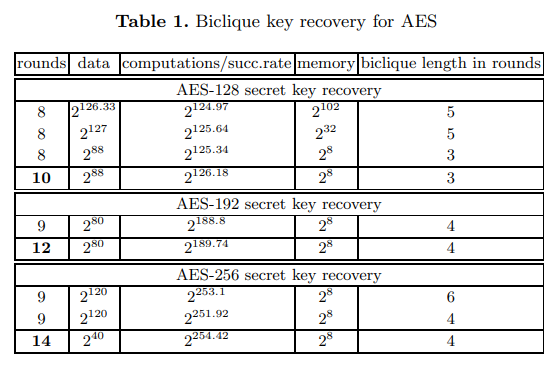
\includegraphics[width=0.5\linewidth]{Biclique.png} \\ Восстановление ключа с помощью метода биклик}
    \end{figure}

В работе \cite{aes6} описываются атаки восстановления секретного ключа, представляющие собой атаки на связанных ключах, на шифры AES с длинами ключей в 192 и 256 бит. При этом используются вариации атаки методом бумеранга. Для атаки на шифр с 192-битным ключом получена оценка временной сложности в $2^{132}$, сложности по памяти --- $2^{152}$; для атаки на шифр с 256-битным ключом получена оценка временной сложности в $2^{99.5}$, сложности по памяти --- $2^{77}$.

В работе \cite{aes3} приводятся описания алгоритмов реализации так называемых квантовых square атак на шифр AES с длиной ключа, равной 128 битам, с 6 раундами, а также на шифр с длиной ключа в 192 бита с 7 раундами.

В статье \cite{aes4} авторами представляется реализация аппаратной архитектуры шифра AES и использованием программируемых пользователем вентильных матриц (FPGA) --- реализация происходила на XCV600, архитектура описывалась с помощью VHDL.  Для представленной в работе реализации на проведенных тестах была определена пропускная способность шифрования и расширования, равная 352 Мбит/с. 

В статье \cite{aes5} авторами описывается реализация программного обеспечения шифра AES, которая обеспечивает высокую скорость на различных типах архитектур процессоров. Рассматриваются методы уменьшения количества инструкций процессора, используемых для шифра AES. В частности, в работе приводятся результаты для таких процессоров, как  Motorola PowerPC G4 7410 (архитектура ppc32), Intel Pentium 4 f12 (архитектура x86), Sun UltraSPARC III (архитектура sparcv9), Intel Core 2 Quad Q6600 6fb (архитектура amd64), AMD Athlon 64 X2 3800+ 15/75/2 (архитектура amd64): для каждого процессора были получены лучшие значения характеристики Цикл/байт, показывающей количество тактовых циклов, которое выполнит процессор на байт данных, обрабатываемый в рассматриваемом алгоритме.

\subsection{Шифр ГОСТ 34.12-2018 Магма}

Описание шифра приводится в соответствии с описанием, приведенным в стандарте \cite{gost}.

На вход алгоритму шифрования подается блок $T$ размером 64 бита и 256-битный ключ $KEY[0], ..., KEY[255]$.

При шифровании блока $T = T_1 \mathbin\Vert T_0$, где $T_1, T_0$ --- 32-битные блоки, используются итерационные ключи $K_1, ..., K_{32}$, а также преобразования $G$ и $g$, которые описаны далее. Схема шифрования может быть описана следующим образом:

\begin{enumerate}
    \item $CT_1 = T_1$; $CT_0 = T_0$

    \item $For$ $i$ $=$ $1$ $to$ $31$ $do$ \{ 

    \hspace{0.5cm} $(CT_{2i+1}, CT_{2i}) = G[K_i](CT_{2i-1}, CT_{2i-2})$;
    
    \}

    \item $CT = (g[K_{32}](CT_{62}) \oplus CT_{63}) \mathbin\Vert CT_{62}$.
    
\end{enumerate}

Зашифрованный блок входного блока $T$ содержится в 64-битном блоке $CT$.


Схема расшифрования зашифрованного блока $CT = CT_1 \mathbin\Vert CT_0$, где $CT_1, CT_0$ --- 32-битные блоки, может быть описана следующим образом:

\begin{enumerate}
    \item $T_1 = CT_1$; $T_0 = CT_0$;

    \item $For$ $i$ $=$ $1$ $to$ $31$ $do$ \{ 

    \hspace{0.5cm} $(T_{2i+1}, T_{2i}) = G[K_{32-i+1}](T_{2i-1}, T_{2i-2})$;
    
    \}

    \item $T = (g[K_{1}](T_{62}) \oplus T_{63}) \mathbin\Vert T_{62}$.
\end{enumerate}

Расшифрованный блок входного блока $CT$ содержится в 64-битном блоке $T$.

Описание компонентов шифра:

\begin{itemize}

    \item Функция $G$ принимает два 32-битных блока $a$ и $b$, имеет 32-битный параметр $k$ и возвращает набор из двух 32-битных блоков $G[k](a, b)$. Данный набор определяется следующим образом: $G[k](a, b) = (b, g[k](b) \oplus a)$. Функция $g$ возвращает 32-битный блок и определяется следующим образом: $g[k](a) = (t(a \boxplus k)) <<< 11$ (через $\boxplus$ обозначена операция сложения по модулю $2^{32}$ соответствующих двоичным строкам $a$ и $k$ десятичных чисел, результатом которой является двоичная запись полученной суммы). Функция $t$ принимает 32-битную строку, также возвращает 32-битный блок и определяется следующим образом: $t(a) = t(a_7 \mathbin\Vert ... \mathbin\Vert a_0) = \pi_7(a_7) \mathbin\Vert ... \mathbin\Vert \pi_0(a_0)$, где $a_7, ..., a_0$ --- 4-битные слова. Перестановки $\pi_0, ..., \pi_7$ представлены в таблице:

    \begin{longtable}{|p{0.5cm}|p{0.5cm}|p{0.5cm}|p{0.5cm}|p{0.5cm}|p{0.5cm}|p{0.5cm}|p{0.5cm}|p{0.5cm}|p{0.5cm}|p{0.5cm}|p{0.5cm}|p{0.5cm}|p{0.5cm}|p{0.5cm}|p{0.5cm}|p{0.5cm}|}
\hline
$\pi_0$ & 12 & 4 & 6 & 2 & 10 & 5 & 11 & 9 & 14 & 8 & 13 & 7 & 0 & 3 & 15 & 1 \\
\hline
$\pi_1$ & 6 & 8 & 2 & 3 & 9 & 10 & 5 & 12 & 1 & 14 & 4 & 7 & 11 & 13 & 0 & 15 \\
\hline
$\pi_2$ & 11 & 3 & 5 & 8 & 2 & 15 & 10 & 13	& 14 & 1 & 7 & 4 & 12 & 9 & 6 & 0 \\
\hline
$\pi_3$ & 12 & 8 & 2 & 1 & 13 & 4 & 15 & 6 & 7 & 0 & 10 & 5 & 3 & 14 & 9 & 11 \\
\hline
$\pi_4$ & 7 & 15 & 5 & 10 & 8 & 1 & 6 & 13 & 0 & 9 & 3 & 14 & 11 & 4 & 2 & 12 \\
\hline
$\pi_5$ & 5 & 13 & 15 & 6 & 9 & 2 & 12 & 10 & 11 & 7 & 8 & 1 & 4 & 3 & 14 & 0 \\
\hline
$\pi_6$ & 8 & 14 & 2 & 5 & 6 & 9 & 1 & 12 & 15 & 4 & 11 & 0 & 13 & 10 & 3 & 7 \\
\hline
$\pi_7$ & 1 & 7 & 14 & 13 & 0 & 5 & 8 & 3 & 4 & 15 & 10	& 6 & 9 & 12 & 11 & 2 \\
\hline
\caption{Перестановки $\pi_0, ..., \pi_7$}
\end{longtable}

    \item Вычисление итерационных ключей --- значений $K_1, ..., K_{32}$ --- происходит на основе ключа $KEY$ по следующему алгоритму:

    \begin{itemize}
        \item $K_1 = KEY[255] \mathbin\Vert ... \mathbin\Vert KEY[224]$;

        \item $K_2 = KEY[223] \mathbin\Vert ... \mathbin\Vert KEY[192]$;

        \item $K_3 = KEY[191] \mathbin\Vert ... \mathbin\Vert KEY[160]$;

        \item $K_4 = KEY[159] \mathbin\Vert ... \mathbin\Vert KEY[128]$;

        \item $K_5 = KEY[127] \mathbin\Vert ... \mathbin\Vert KEY[96]$;

        \item $K_6 = KEY[95] \mathbin\Vert ... \mathbin\Vert KEY[64]$;

        \item $K_7 = KEY[63] \mathbin\Vert ... \mathbin\Vert KEY[32]$;

        \item $K_8 = KEY[31] \mathbin\Vert ... \mathbin\Vert KEY[0]$;

        \item $K_{i+8} = K_i$, где $i = 1, 2, ..., 8$;

        \item $K_{i+16} = K_i$, где $i = 1, 2, ..., 8$;

        \item $K_{i+24} = K_{9-i}$, где $i = 1, 2, ..., 8$;
        
    \end{itemize}
\end{itemize}

\subsection{Шифр ГОСТ 34.12-2018 Кузнечик}

Описание шифра приводится в соответствии с описанием, приведенным в стандарте \cite{gost}.

На вход алгоритму шифрования подается блок $T$ размером 128 бит и 256-битный ключ $KEY[0], ..., KEY[255]$.

При шифровании используются итерационные ключи $K_1, ..., K_{10}$, а также преобразования $S$ и $L$, которые описаны далее. Схема шифрования может быть описана следующим образом:

\begin{enumerate}
    \item $CT_1 = T$;

    \item $For$ $i$ $=$ $1$ $to$ $9$ $do$ \{ 

    \hspace{0.5cm} $CT_{i+1} = L(S(K_i \oplus CT_{i}))$;
    
    \}

    \item $CT = K_{10} \oplus CT_{10}$.
    
\end{enumerate}

Зашифрованный блок входного блока $T$ содержится в 128-битном блоке $CT$.


Схема расшифрования зашифрованного блока $CT$ может быть описана следующим образом:

\begin{enumerate}
    \item $T_{10} = CT$;

    \item $For$ $i$ $=$ $10$ $downto$ $2$ $do$ \{ 

    \hspace{0.5cm} $T_{i-1} = S^{-1}(L^{-1}(K_i \oplus T_{i}))$;
    
    \}

    \item $T = K_{1} \oplus T_1$.
\end{enumerate}

Расшифрованный блок входного блока $CT$ содержится в 128-битном блоке $T$.

Описание компонентов шифра:

\begin{itemize}

    \item Функция $S$ принимает блок $a$ размером 128 бит и возвращает блок $S(a)$ такого же размера. Блок $S(a)$ определяется следующим образом: $S(a) = S(a_{15}\mathbin\Vert ... \mathbin\Vert a_0) = \pi(a_{15}) \mathbin\Vert ... \mathbin\Vert \pi(a_0)$, где $a_{15}, ..., a_0$ --- однобайтовые блоки.

    Перестановка $\pi$ определена на множестве целых чисел $\{ 0, ..., 255\}$. Данная перестановка принимает 8-битную строку $a$, по десятичному значению которой по таблице перестановки $\pi$ ниже определяется десятичное значение $\pi(a)$, двоичная запись которого и возвращается данной перестановкой.

    \begin{longtable}{|p{0.5cm}|p{0.5cm}|p{0.5cm}|p{0.5cm}|p{0.5cm}|p{0.5cm}|p{0.5cm}|p{0.5cm}|p{0.5cm}|p{0.5cm}|p{0.5cm}|p{0.5cm}|p{0.5cm}|p{0.5cm}|p{0.5cm}|p{0.5cm}|}
    \hline
    252 & 238 & 221 & 17 & 207 & 110 & 49 & 22 & 251 & 196 & 250 & 218 & 35 & 197 & 4 & 77 \\ 
    \hline
    233 & 119 & 240 & 219 & 147 & 46 & 15 & 186 & 23 & 54 & 241 & 187 & 20 & 205 & 95 & 193 \\
    \hline
    249 & 24 & 101 & 90 & 226 & 92 & 239 & 33 & 129 & 28 & 60 & 66 & 139 & 1 & 142 & 79 \\ 
    \hline
    5 & 132 & 2 & 174 & 227 & 106 & 143 & 160 & 6 & 11 & 237 & 152 & 127 & 212 & 211 & 31 \\
    \hline
    235 & 52 & 44 & 81 & 234 & 200 & 72 & 171 & 242 & 42 & 104 & 162 & 253 & 58 & 206 & 204 \\ 
    \hline
    181 & 112 & 14 & 86 & 8 & 12 & 118 & 18 & 191 & 114 & 19 & 71 & 156 & 183 & 93 & 135 \\
    \hline
    21 & 161 & 150 & 41 & 16 & 123 & 154 & 199 & 243 & 145 & 120 & 111 & 157 & 158 & 178 & 177 \\
    \hline
    50 & 117 & 25 & 61 & 255 & 53 & 138 & 126 & 109 & 84 & 198 & 128 & 195 & 189 & 13 & 87 \\
    \hline
    223 & 245 & 36 & 169 & 62 & 168 & 67 & 201 & 215 & 121 & 214 & 246 & 124 & 34 & 185 & 3 \\
    \hline
    224 & 15 & 236 & 222 & 122 & 148 & 176 & 188 & 220 & 232 & 40 & 80 & 78 & 51 & 10 & 74 \\
    \hline
    167 & 151 & 96 & 115 & 30 & 0 & 98 & 68 & 26 & 184 & 56 & 130 & 100 & 159 & 38 & 65 \\
    \hline
    173 & 69 & 70 & 146 & 39 & 94 & 85 & 47 & 140 & 163 & 165 & 125 & 105 & 213 & 149 & 59 \\
    \hline
    7 & 88 & 179 & 64 & 134 & 172 & 29 & 247 & 48 & 55 & 107 & 228 & 136 & 217 & 231 & 137 \\
    \hline
    225 & 27 & 131 & 73 & 76 & 63 & 248 & 254 & 141 & 83 & 170 & 144 & 202 & 216 & 133 & 97 \\
    \hline
    32 & 113 & 103 & 164 & 45 & 43 & 9 & 91 & 203 & 155 & 37 & 208 & 190 & 229 & 108 & 82 \\
    \hline
    89 & 166 & 116 & 210 & 230 & 244 & 180 & 192 & 209 & 102 & 175 & 194 & 57 & 75 & 99 & 182 \\
    \hline
    \caption{Таблица перестановки $\pi$}
    \end{longtable}


    \item Функция $L$ принимает блок $a$ размером 128 бит и возвращает блок $L(a)$ такого же размера. Блок $L(a)$ определяется следующим образом: $L(a) = R^{16}(a)$, где $R(a) = R(a_{15} \mathbin\Vert ... \mathbin\Vert a_0) = l(a_{15}, ..., a_0) \mathbin\Vert a_{15} \mathbin\Vert ... \mathbin\Vert a_1 $, где $a_{15}, ..., a_0$ --- однобайтовые блоки, а $R^{16}$ обозначает последовательное применение функции $R$ 16 раз. 
    
    Функция $l$ принимает 16 8-битных слов $a_{15}, ..., a_0$ и определяется следующим образом: $l(a_{15}, ..., a_0) = \Delta^{-1}(148\Delta(a_{15}) + 32\Delta(a_{14}) + 133\Delta(a_{13}) + 16\Delta(a_{12}) + 194\Delta(a_{11}) + 192\Delta(a_{10}) + \Delta(a_{9}) + 251\Delta(a_{8}) + \Delta(a_{7}) + 192\Delta(a_{6}) + 194\Delta(a_{5}) + 16\Delta(a_{4}) + 133\Delta(a_{3}) + 32\Delta(a_{2}) + 148\Delta(a_{1}) + \Delta(a_{0}))$, где функция $\Delta$ отображает битовую строку $z_7 \mathbin\Vert ... \mathbin\Vert z_0$ в число поля $GF(2)[x]/p(x)$, где $p(x) = x^8 + x^7 + x^6 + x + 1$, соответствующее многочлену $z_0 + z_1\theta + ... + z_7\theta^7$. Все операции сложения и умножения осуществляются в поле $GF(2)[x]/p(x)$.

    \item Вычисление итерационных ключей --- значений $K_1, ..., K_{10}$ --- происходит на основе ключа $KEY$ по следующему алгоритму:

    \begin{enumerate}
        \item $K_1 = KEY[255] \mathbin\Vert ... \mathbin\Vert KEY[128]$; $K_2 = KEY[127] \mathbin\Vert ... \mathbin\Vert KEY[0]$;

        \item $For$ $i$ $=$ $1$ $to$ $4$ $do$ \{ 

        \hspace{0.5cm} $(K_{2i + 1}, K_{2i + 2}) = F[C_{8(i-1) + 8}]...F[C_{8(i-1) + 1}](K_{2i-1}, K_{2i})$;
    
        \}
        
    \end{enumerate}

    При вычислении итерационных ключей используются значения $C_i = L(a_i)$, где $i = 1, 2, ..., 32$, $a_i$ --- двоичное представление соответствующего целого числа $i$. Также используется функция $F[k](a, b)$, принимающая две 128-битные строки $a$ и $b$, имеющая 128-битный параметр $k$, которая возвращает набор из двух значений, который определяется следующим образом: $F[k](a, b) = (L(S(k \oplus b)) \oplus a, b)$.
    
\end{itemize}

\subsection{Шифры IDEA и IDEA NXT}

\subsubsection{Шифр IDEA}
Описание шифра IDEA приводится в соответствии со статьей \cite{idea} авторов данного шифра.

На вход алгоритму шифрования подается 64-битный блок $T = X_1 \mathbin\Vert X_2 \mathbin\Vert X_3 \mathbin\Vert X_4$, где $X_1, X_2, X_3, X_4$ --- блоки длины 16 бит, и 128-битный секретный ключ KEY.

Схема шифра IDEA представлена на рисунке ниже:

    \begin{figure}[h!]
    \center{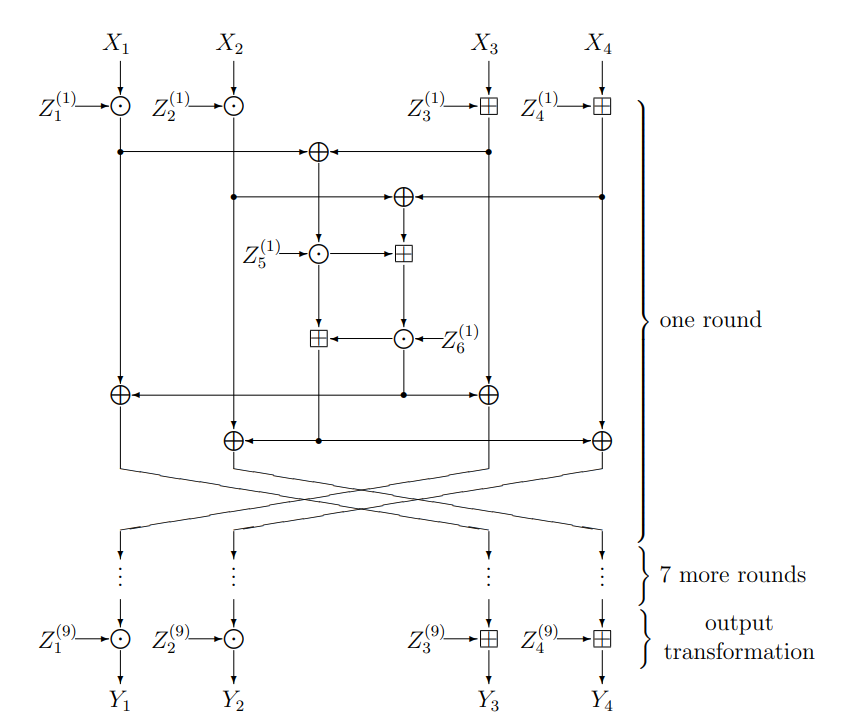
\includegraphics[width=0.5\linewidth]{idea.png} \\ Схема шифра IDEA}
    \end{figure}

Зашифрованный блок $CT$ определяется следующим образом: $CT = Y_1 \mathbin\Vert Y_2 \mathbin\Vert Y_3 \mathbin\Vert Y_4$, где $Y_1, Y_2, Y_3, Y_4$ --- блоки длины 16 бит.

В алгоритме используются 52 раундовых ключа $Z_i^{(j)}$, где $1 \leq i \leq 6$ при $1 \leq j \leq 8$ и $1 \leq i \leq 4$ при $j = 9$ (по 6 на каждый раун шифрования и 4 для выходного преобразования), которые получаются из секретного ключа KEY следующим образом: ключ KEY разделяется на 8 блоков длины 16 бит, после чего раундовые ключи инициализируются данными блоками в следующем порядке (после инициализации восьмым блоком дальнейшая инициализация происходит снова с первого блока секретного ключа): $Z_1^{(1)}, ..., Z_6^{(1)}; Z_1^{(2)}, ..., Z_6^{(2)}; ...; Z_1^{(8)}, ..., Z_6^{(8)}; Z_1^{(9)}, ..., Z_4^{(9)}$.

Схема расшифровки шифротекста аналогична схеме шифрования, за исключением того, что используются другие раундовые ключи. Порядок ключей следующий:
$Z_1^{(9)^{-1}}, Z_2^{(9)^{-1}}, -Z_3^{(9)}, -Z_4^{(9)}, Z_5^{8}, Z_6^{8}$; ...; $Z_1^{(2)^{-1}}, Z_2^{(2)^{-1}}, -Z_3^{(2)}, -Z_4^{(2)}, Z_5^{1}, Z_6^{1}$; $Z_1^{(1)^{-1}}, Z_2^{(1)^{-1}}, -Z_3^{(1)}, -Z_4^{(1)}$. При этом элемент $Z^{-1}$ обозначает обратный элемент к $Z$ по модулю $2^{16} + 1$.


\subsubsection{Шифр IDEA NXT}
Описание шифра IDEA NXT (ранее известного как FOX) приводится в соответствии со статьей \cite{fox} авторов данного шифра.

Авторами определяются следующие варианты шифров семейства IDEA NXT (далее будет использоваться ранее имя данного шифра --- FOX):

\begin{enumerate}
    \item FOX64 --- 64-битный блок; 128-битный ключ; 16 раундов шифрования;
    \item FOX128 --- 128-битный блок; 256-битный ключ; 16 раундов шифрования;
    \item FOX64$/k/r$ --- 64-битный блок; $k$-битный ключ, $0 \leq k \leq 256$, $k$ кратно 8; $12 \leq r \leq 255$ раундов шифрования;
    \item FOX128$/k/r$ --- 128-битный блок; $k$-битный ключ, $0 \leq k \leq 256$, $k$ кратно 8; $12 \leq r \leq 255$ раундов шифрования.
\end{enumerate}

При шифровании 64-битного блока $T$ происходят следующие действия:

$CT = lmid64(lmor64(...(lmor64(T, RK_0), ..., RK_{r-2}), RK_{r-1}$), где $RK = RK_0 \mathbin\Vert ... \mathbin\Vert RK_{r-1}$ --- поток полученных из секретного ключа раундовых 64-битных ключей.

При рашифровании 64-битного блока $CT$ происходят следующие действия:

$T = lmid64(lmio64(...(lmio64(T, RK_{r-1}), ..., RK_{1}), RK_{0}$).

При 128-битном шифровании вместо функций $lmor64, lmid64$ и $lmio64$ используются соответственно функции $elmor128, elmid128$  и $elmio128$.

Описаний компонентов шифра:

\begin{itemize}
    \item Схемы функций $lmor64$ и $elmor128$ приведены на рисунке далее:
    
    \begin{figure}[h!]
    \center{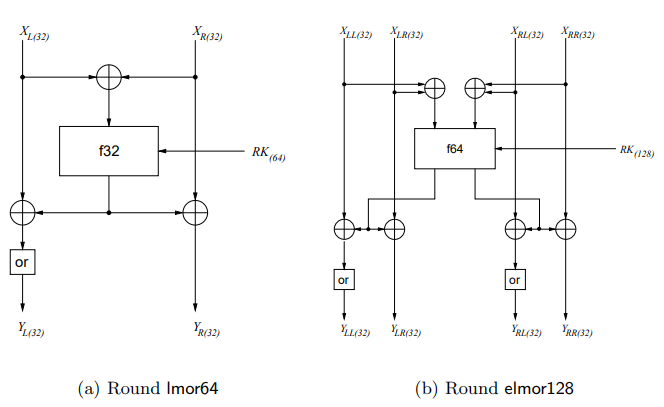
\includegraphics[width=0.7\linewidth]{fox1.png} \\ Схема функций $lmor64$ и $elmor128$}
    \end{figure}

    \item Функции $lmid64, lmio64$ определяются аналогичным образом, но функция $or$ заменяется на тождественную функцию и функцию $io$ соответственно;

    \item Функции $elmid128, elmio128$ определяются аналогичным образом, но функции $or$ заменяются на тождественные функции и функции $io$ соответственно;

    \item Функция $or$ принимает 32-битовый блок $X$ и возвращает 32-битовый блок $Y$ по следующему правилу: $Y_0 \mathbin\Vert Y_1 = X_1 \mathbin\Vert (X_0 \oplus X_1)$; Функция $io$ есть обратная функция к функции $or$;

    \item Функция $f_{32}$ принимает на вход 32-битный блок $X$, 64-битный раундовый ключ $RK = RK_0 \mathbin RK_1$, где $RK_0, RK_1$ --- 32-битные блоки, и возвращает 32-битный блок $Y = sigma4(mu4(sigma4(X, RK_0)) \oplus RK_1)\oplus RK_0$;

    \item Функция $f_{64}$ принимает на вход 64-битный блок $X$, 128-битный раундовый ключ $RK = RK_0 \mathbin RK_1$, где $RK_0, RK_1$ --- 64-битные блоки, и возвращает 64-битный блок $Y = sigma8(mu8(sigma8(X, RK_0)) \oplus RK_1)\oplus RK_0$;

    \begin{figure}[h!]
    \center{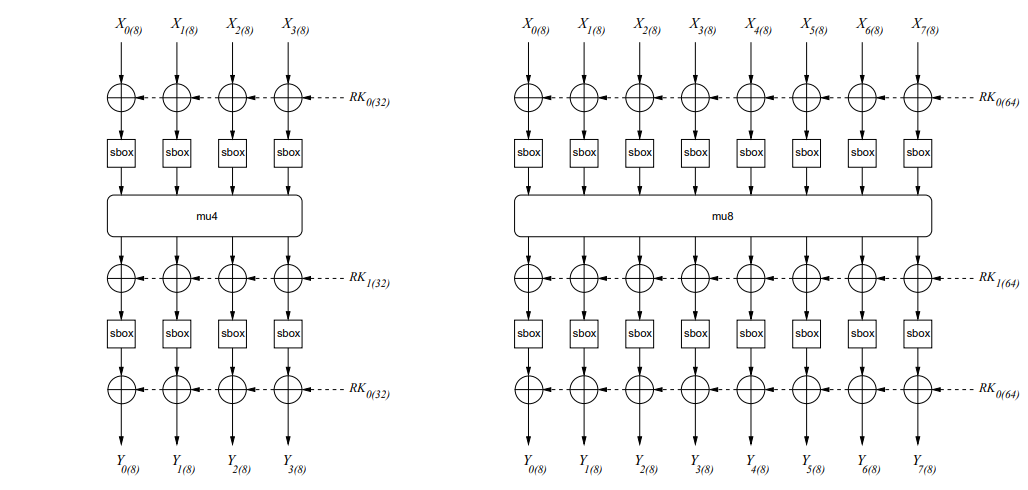
\includegraphics[width=0.7\linewidth]{fox2.png} \\ Схема функций $f32$ и $f64$}
    \end{figure}

    \item Преобразования $sigma4$ и $sigma8$ определяются S-блоком, приведенным ниже: по первой цифре шестнадцатеричного представления выбирается номер строки, по второй --- номер столбца. Число, стоящее на пересечении выбранных строки и столбца, возвращается после обращения к функции данной функции.

    \begin{figure}[h!]
    \center{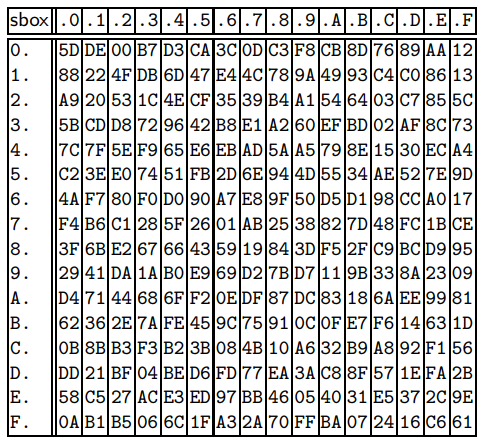
\includegraphics[width=0.4\linewidth]{fox3.png} \\ S-блок, определяющий преобразование $sigma$}
    \end{figure}

    \item Функции $mu4$ и $mu8$ принимают 32-битный или, соответственно, 64-битный блок $X = X_0 \mathbin\Vert ... \mathbin\Vert X_n$, где $X_0, ..., X_n$ --- 8-битные блоки, и производит их умножение на некоторые заданные матрицы.

    \item Алгоритм обработки секретного ключа и выработки раундовых ключей

    В зависимости от используемого вариант шифра может использоваться одна из схем выработки раундового ключа: $NL64$ --- 64-битный блок, ключ размера $0 \leq k \leq 128$ бит; $NL64h$ --- 64-битный блок, ключ размера $136 \leq k \leq 256$ бит; $NL128$ --- 128-битный блок, ключ размера $0 \leq k \leq 256$ бит. Данные схемы представлены на рисунке далее.

    \begin{figure}[h!]
    \center{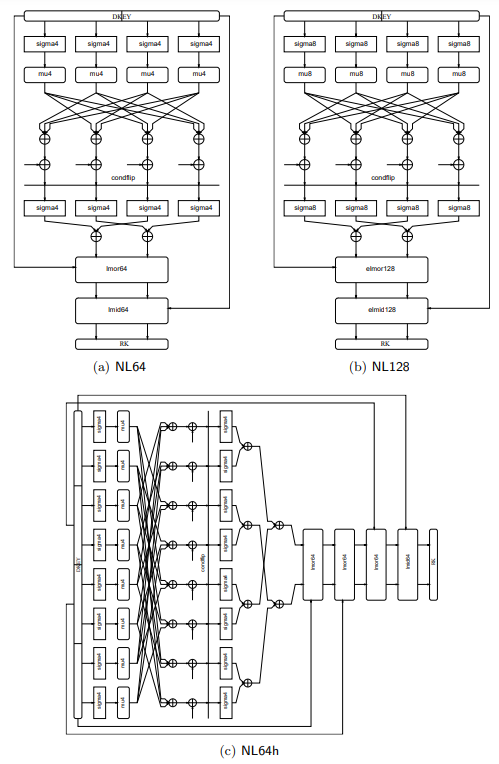
\includegraphics[width=0.6\linewidth]{fox4.png} \\ Схемы алгоритмов выработки раундового ключа для разных вариантов шифра}
    \end{figure}

    При этом для определения поступающих для выработки раундового ключа битов секретного ключа $KEY$ функцией $DKEY$ используется 24-битный регистр сдвига с линейной обратной связью.
    
\end{itemize}

\subsection{Шифр RC6}

Описание шифра RC6 приводится на основе работы \cite{rc6} авторов данного шифра.

Для конкретной спецификации шифра RC6 принято использовать обозначение RC6-$w/r/b$, где $w$ обозначает размер битового слова, $r$ обозначает количество раундов шифрования и расшифрования, а $b$ --- длину секретного ключа в байтах (от 0 до 255 включительно).  

Предварительные действия:

\begin{enumerate}
    \item Вводится секретный ключ $KEY = KEY[0] \mathbin\Vert ... \mathbin\Vert KEY[b-1]$ длины $b$ байт;

    \item Ключ копируется в массив $L[0], ..., L[c-1]$, состоящий из $c =\lceil \frac{8b}{w} \rceil$ $w$-битных слов. При необходимости $L[c-1]$ дополняется незначащими нулями;

    \item Определяется массив $w$-битовых раундовых ключей $S[0], ..., S[2r+3]$, непосредственно используемых при шифровании и расшифровании:

    \begin{enumerate}
        \item $S[0] = P_{w}$;

        \item $For$ $i$ $=$ $1$ $to$ $2r + 3$ $do$ \{ 

        \hspace{0.5cm} $S[i] = S[i-1] + Q_{w}$;
    
        \}

        \item $A = 0$; $B = 0$; $i = 0$; $j = 0$;

        \item $q = 3\cdot \max\{c, 2r + 4\}$;

        \item $For$ $s$ $=$ $1$ $to$ $q$ $do$ \{ 

        \hspace{0.5cm} $A = S[i] = (S[i] + A + B) <<< 3$;

        \hspace{0.5cm} $B = L[j] = (L[j] + A + B) <<< (A + B)$;

        \hspace{0.5cm} $i = (i + 1) \mod (2r + 4)$;

        \hspace{0.5cm} $j = (j + 1) \mod (c)$;
    
        \}
    \end{enumerate}
    При этом используются значения $P_w$ и $Q_w$, вычисляемые следующим образом: $Q_w = Odd((f - 1)2^w)$, \\$P_w~=~Odd((e~-~2)2^w)$, где $f$ --- число Фибоначчи (золотое сечение), $e$ --- основание натурального логарифма, функция $Odd$ ---  округление до ближайшего нечетного целого числа.
\end{enumerate}

При шифровании выполняется следующая последовательность действий:

\begin{enumerate}
    \item Блок текста длины $4w$ сохраняется в $w$-битных регистрах $A, B, C, D$: $T = A \mathbin\Vert B \mathbin\Vert C \mathbin\Vert D$;

    \item $B = B + S[0]$; $D = D + S[1]$;

    \item $For$ $i$ $=$ $1$ $to$ $r$ $do$ \{ 

    \hspace{0.5cm} $t = B(2B + 1) <<< log_2(w)$;
    
    \hspace{0.5cm} $u = D(2D + 1) <<< log_2(w)$;

    \hspace{0.5cm} $A = ((A \oplus t) <<< u) + S[2i]$;

    \hspace{0.5cm} $C = ((C \oplus u) <<< t) + S[2i + 1]$;

    \hspace{0.5cm} $A = B$; $B = C$; $C = D$; $D = A$;
    
\}

    \item $A = A + S[2r + 2]$; $C = C + S[2r + 3]$;

    \item Зашифрованный блок $CT = A \mathbin\Vert B \mathbin\Vert C \mathbin\Vert D$.
    
\end{enumerate}

При расшифровании выполняется следующая последовательность действий:

\begin{enumerate}
    \item Зашифрованный блок длины $4w$ сохраняется в $w$-битных регистрах $A, B, C, D$: $CT = A \mathbin\Vert B \mathbin\Vert C \mathbin\Vert D$;
    
    \item $C = C - S[2r + 3]$; $A = A - S[2r + 2]$;

    \item $For$ $i$ $=$ $r$ $downto$ $1$ $do$ \{ 

    \hspace{0.5cm} $A = D$; $B = A$; $C = B$; $D = C$;

    \hspace{0.5cm} $u = D(2D + 1) <<< log_2(w)$;
    
    \hspace{0.5cm} $t = B(2B + 1) <<< log_2(w)$;

    \hspace{0.5cm} $C = ((C - S[2i + 1]) >>> t) \oplus u$;

    \hspace{0.5cm} $A = ((A - S[2i]) >>> u) \oplus t$;
    
\}

    \item $D = D - S[1]$; $B = B - S[0]$;

    \item Расшифрованный блок $T = A \mathbin\Vert B \mathbin\Vert C \mathbin\Vert D$.
\end{enumerate}

Все арифметические операции выполняются по модулю $2^w$; циклические сдвиги содержимого слова $a$ при выполнении операции $a <<< b$ или $a >>> b$ выполняются на величину, определяемую младшими $log_2(w)$ битами $b$.

\section{Заключение}

В работе были описаны основные блоковые шифры: DES, 3DES, AES, ГОСТ 34.12-2018 Магма, ГОСТ 34.12-2018 Кузнечик, IDEA, IDEA NXT и RC6. Также более подробно был рассмотрен шифр AES. Для данного шифра известно большое число теоретических атак с использованием самых различных методов компрометации секретного ключа. Отдельно стоит отметить так называемые атаки по побочным каналам, как, например, атака, основанная на анализе времени выполнения операции шифрования, теоретически позволяющая раскрыть информацию об используемом секретном ключе. Описанные теоретические атаки не выглядят практичными. При этом на данный момент не известно какой бы то ни было практической атаки, которая позволила бы извлечь зашифрованные шифром AES данные, не обладая знанием секретного ключа.


\end{document}
